\documentclass[a4paper,12pt,titlepage,oneside]{article}

\title{Cubic Curves Over Finite Fields}
\author{Will Bolton}
\date{\today}
\bibliographystyle{abbrv}
% Package input
\usepackage[textwidth=15cm,textheight=23cm]{geometry}
\usepackage{graphicx}
\usepackage{natbib}
\usepackage{amsmath}
\usepackage{amssymb}
\usepackage{amsfonts}
\usepackage{tikz}
\usepackage{color}
\usepackage{cleveref}
\usepackage{lipsum}
\usepackage{microtype}
\usepackage{enumerate}
\usepackage{listings}

% Proof environment
\newenvironment{proof}
 {
   \begin{trivlist}
     \item[] {\bf Proof.}
 }
 {
    \nolinebreak
    \hfill
    \rule{2mm}{2mm}
   \end{trivlist}
 }
 
% Sketch of proof environment
\newenvironment{sproof}
{
   \begin{trivlist}
     \item[] {\bf Sketch of proof.}
 }
{
    \nolinebreak
    \hfill
    \rule{2mm}{2mm}
   \end{trivlist}
}
 
% Definition environment
\newenvironment{definition}
 {
   \begin{trivlist}
     \item[] {\bf Definition.}
 }
 {
   \end{trivlist}
 }
 
% Theorem environment (this is a bit different because there is a \newtheorem command)
% Syntax \newtheorem{ <<name>> }{ <<Displayed Title>> }[ <<Where to take numbering from>> ]
\newtheorem{theorem}{Theorem}[subsection]
\newtheorem{lemma}{Lemma}[subsection]
\newtheorem{proposition}{Proposition}[subsection]
\newtheorem{corollary}{Corollary}[subsection]

% Custom commands
\newcommand{\ud}{\, {\rm d} \kern-.015em }
\newcommand{\bm}[1]{\mbox{\protect\boldmath $ #1 $}}
\newcommand{\Q}{\mathbb{Q}}
\newcommand{\R}{\mathbb{R}}
\newcommand{\N}{\mathbb{N}}
\newcommand{\Z}{\mathbb{Z}}
\newcommand{\an}[1][n]{\mathbb{A}^{#1}}
\newcommand{\pn}[1][n]{\mathbb{P}^{#1}}
\newcommand{\fp}[1][p]{\mathbb{F}_{#1}}
\newcommand{\zn}[1][n]{\mathbb{Z}_{#1}}
\newcommand{\fpu}[1][p]{\mathbb{F}_{#1}^{\times}}
\newcommand{\for}{\text{for }}
\newcommand{\si}{\text{if }}
\newcommand{\pai}{\mathcal{O}}
\newcommand{\galt}[1]{{#1}_{\ast}} % alternate characters for gauss proof

% Define colours for listings appendix
\definecolor{dkgreen}{rgb}{0,0.6,0}
\definecolor{gray}{rgb}{0.5,0.5,0.5}
\definecolor{mauve}{rgb}{0.58,0,0.82}

% Define other settings for listings appendix. Taken from tex.sx, I think
\lstset{frame=none,
  language=Python,
  aboveskip=0pt,
  belowskip=0pt,
  showstringspaces=false,
  columns=flexible,
  basicstyle={\small\ttfamily},
  numbers=left,
  numberstyle=\tiny\color{gray},
  keywordstyle=\color{blue},
  commentstyle=\color{dkgreen},
  stringstyle=\color{mauve},
  breaklines=false,
  breakatwhitespace=true,
  tabsize=3
}


\begin{document}
\begin{titlepage}
	\centering
	% \includegraphics[width=0.15\textwidth]{example-image-1x1}\par\vspace{1cm}
	{\scshape\LARGE Lancaster University \par}
	\vspace{1cm}
	{\scshape\Large MSci Mathematics Dissertation\par}
	\vspace{1.5cm}
	{\huge\bfseries Cubic Curves Over Finite Fields\par}
	\vspace{2cm}
	{\Large\itshape William Bolton\par}
	\vfill
	supervised by\par
	Dr.~Nadia \textsc{Mazza}

	\vfill

% Bottom of the page
	{\large \today\par}
\end{titlepage}
\tableofcontents
\clearpage

\section*{Motivation}
\addcontentsline{toc}{section}{Motivation}
This is the motivation for my dissertation.

\clearpage

\section{Prerequisites}
\label{prerequisite-section}
\subsection{Finite fields}
% Going to include linear congruences in this section too
\begin{definition}
	A field is a commutative, unital ring in which every non-zero element is invertible
\end{definition}
Recall the group $\zn$, the group of integers modulo some natural number $n$.
For a given $n$, we have already seen that we can make $\zn$ a ring by defining the natural multiplication law.
However, the ring $\zn$ is a field if and only if $n$ is prime, and this is denoted by writing $\zn = \fp$ to emphasise both that the modulus is prime and that the ring is a field.
The reason this is true is obvious when considering inverses; if we attempt to make a field out of $\zn[4]$, we find that $2$ has no inverse, since
\begin{align*}
	2 \times 0 &= 0\\
	2 \times 1 &= 2\\
	2 \times 2 &= 0\\
	2 \times 3 &= 2.
\end{align*}
Therefore, $\zn[4]$ fails to meet the criteria for a field.

The question of finding inverses, you should also remember, has an easy, general solution, which involves the euclidean algorithm, which is recapped here.
\begin{definition}
	A linear congruence is an equation of the form
	$$ax \equiv b \mod n$$
\end{definition}
Recall this basic definition from \texttt{MATH111}. Clearly, the nature of linear congruences lends itself to arithmetic within finite fields.

\subsection{The projective plane}
\subsubsection{Affine Space and Affine Curves}
The main object of interest in this subsection is the projective plane.
Before we introduce it, though, we begin with a prerequisite definition.

\begin{definition}
	Let $k$ be an algebraically closed field. Define affine $n$-space, or $\an$, to be the set of all $n$-tuples, or points,
	$$\an = \{ (a_1,a_2,\ldots,a_n) | a_i \in k\}.$$
\end{definition}

The consideration of algebraically closed fields differentiates affine space from $\R^n$, where from now on, unless otherwise mentioned, we take the field $k = \C$.
% note about how we don't need to use C necessarily?
We call affine 2-space, or $\an[2]$, the \emph{affine plane}.

In affine $n$-space, it is possible to define \emph{affine curves} in the following way.
\begin{definition}
	In $\an$, for a given polynomial $f$ in $n$ variables $x_1,\ldots,x_n$, an \emph{affine curve} is the set $V(f)$ of all points $(x_1,\ldots,x_n)$ such that $f(x_1,\ldots,x_n)=0$. More concisely,
	$$V(f) = \{(x_1,\ldots,x_n) | f(x_1,\ldots,x_n)=0$$
\end{definition}
\Cref{affinecurveexample} shows an example of an affine curve.

% unfinished diagram
\begin{figure}[htbp]
	\centering
	\begin{tikzpicture}[scale=0.5,domain=-5:5]
		% axes
		\draw[->] (-5,0) -- (5,0);
		\draw[->] (0,-5) -- (0,5);
		\node [right] at (5,0) {$x$};
		\node [right] at (0,5) {$y$};
		% graph
		\draw 
		plot (\x, {\x});
	\end{tikzpicture}
	\caption{The affine curve $x^3 - 2xy = 0$ in the visible part of $\an[2]$}
	\label{affinecurveexample}
\end{figure}

It is important to distinguish the two objects $V(f)$ and $f$, as $f$ is simply a polynomial, whereas $V(f)$ is the set of points that are a solution to a polynomial \emph{equation} $f(x_1,\ldots,x_n)=0$.
However, for convenience, we write the curve $V(f)$ as its defining polynomial equation $f(x,y)=0$, when it is clear to do so.
The distinction of objects remains, though, and this is purely notational.

More points on notation are that in the affine plane, instead of $x_1$ and $x_2$, we write $x$ and $y$, lowercase.
We also write polynomials as lowercase letters $f$, $g$ etc.
The reason for this will be explained shortly.
\subsubsection{Projective Space}
Now that affine space has been introduced, we are ready to introduce projective $n$-space $\pn$, and with that, the projective plane $\pn[2]$.

The projective plane is an idea that grew out of the renaissance study of perspective in art.
For example, when stood between two railway lines, they appear to meet at the horizon.
\Cref{projective-parallel} is a diagram of the situation.
While this is merely a trick of perspective in euclidean space, in the projective plane, parallel lines \emph{do} meet, at a so called `point at infinity'.
% euclidean/affine? What?
The idea is to add these points at infinity to the affine plane so that each line contains exactly one.
On top of this is the one exception, the `line at infinity', which is defined to be the unique line that is simply the collection of all points at infinity.
These ideas, while formative, are not rigorous, and we present the proper definition and constructions (there are two) of projective space below.

\begin{figure}[htbp]
	\centering
	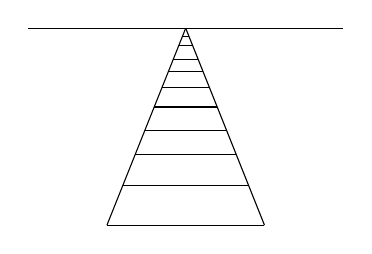
\begin{tikzpicture}[scale=0.5]
		% railway lines
		\draw (-2,0) -- (0,5);
		\draw (2,0) -- (0,5);
		% sleepers. To work out an appropriate x for given y, x=2(1-(y/5))
		\draw (-2,0) -- (2,0);
		\draw (-1.6,1) -- (1.6,1);
		\draw (-1.28,1.8) -- (1.28,1.8);
		\draw (-1.04,2.4) -- (1.04,2.4);
		\draw (-0.8,3) -- (0.8,3);
		\draw (-0.6,3.5) -- (0.6,3.5);
		\draw (-0.44,3.9) -- (0.44,3.9);
		\draw (-0.32,4.2) -- (0.32,4.2);
		\draw (-0.18,4.55) -- (0.18,4.55);
		\draw (-0.08,4.8) -- (0.08,4.8);
		% horizon
		\draw (-4,5) -- (4,5);
	\end{tikzpicture}
	\caption{Parallel lines `meeting' at infinity in euclidean space}
	\label{projective-parallel}
\end{figure}

% \begin{definition}
% 	The projective plane is an extension of the affine plane $\an[2]$ created by adding `points at infinity' such that every pair of lines intersects exactly once.
% 	Points in projective $n$-space are represented by $n+1$-tuples modulo an equivalence relation, such that not all coordinates are zero.
% \end{definition}

The two constructions of projective space give two different interpretations of it, both of which are useful to consider.
Projective $n$-space can be thought of as either affine $n$-space with points at infinity added (mentioned already) or as a quotient of affine $(n+1)$-space.

\subsubsection{Construction 1: Quotient of $\an[n+1]$}
Remove the origin (i.e. the point $(0,0,\ldots,0)$) from $\an[n+1]$ and define an equivalence relation $\sim$ on the remaining points as follows:
$$(a_0,a_1,\ldots,a_n) \sim (b_0,b_1,\ldots,b_n) \iff (a_0,a_1,\ldots,a_n) = \lambda(b_0,b_1,\ldots,b_n)$$
where $\lambda$ is a non-zero scalar in $\C$. Then we have 
$$\pn = (\an[n+1]\setminus\{(0,\ldots,0)\})/\sim,$$
the set of equivalence classes of $\sim$.

Therefore, we see that points in $\pn$ are equivalence classes of lines in $\an[n+1] \setminus \{0\}$.
For points in $\pn$, write $P = [p_0,p_1,\ldots,p_n]$, where the square brackets represent the \emph{homogeneous coordinates} of the point.
We see that $[p_0,p_1,\ldots,p_n] = \{(\lambda a_0, \lambda a_1,\ldots,\lambda a_n | \lambda \in \C\}$.

By the nature of this construction, it is clear that scaling homogeneous coordinates results in coordinates of the same point.
Therefore, for a given point, there is no unique representation in homogeneous coordinates, and we may scale coordinates for our convenience.

\subsubsection{Construction 2: Extension of $\an[n]$}
Now we present the second construction of $\pn$, which can be thought of as adding points at infinity to affine $n$-space.
This is done inductively on $n$ by defining maps $\alpha_n$ and $\beta_n$.
To begin with, let $\pn[0] = \an[1] \setminus \{0\}$ and let
\begin{alignat*}{2}
&\alpha_n : \an \rightarrow \pn,\quad &&\alpha_n(x_1,\ldots,x_n) = [x_1,\ldots,x_n,1]\\
 &\beta_n : \pn[n-1] \rightarrow \pn,\quad &&\beta_n[X_1,\ldots,X_n] = [X_1,\ldots,X_n,0]
\end{alignat*}
Then we can define
$$\pn = \alpha_n(\an) \cup \beta_n(\pn[n-1])$$
Effectively, we have that $\alpha_n$ is the embedding of affine space in $\pn$ and $\beta_n$ represents the points at infinity of $\pn$.
Notice that the image of $\beta_n$ will always give valid homogeneous coordinates, as we removed zero from $\pn[0]$, and therefore at least one of the first $n$ coordinates will be nonzero.
\subsubsection{Homogenisation of Polynomials}
Now that projective space has been introduced, it is natural to wonder what form curves in projective space take.
If we try to define projective curves in $\pn$ in the same way as affine curves, i.e. as solutions of a polynomial equation $f(x_1,\ldots,x_n)=0$ in $n$ variables, we find that it is not always possible, since we saw that the homogeneous coordinates of a point are not unique.
For example, if we tried to define a projective curve as $F(X,Y,Z)=X^2+Y+Z=0$, we see that $[2,-2,-2]$ is a solution of this equation, and so $[2,-2,-2] \in F$.
However, since we work with homogeneous coordinates, the point $[2,-2,-2]$ is also be written as $[-2,2,2]$, which clearly does not satisfy $F(X,Y,Z)=0$.
This is a problem, as we do not want the representation of a point to affect whether it lies on a curve or not.

To that extent, when working with the projective plane, it is convenient to define a homogeneous polynomial as a polynomial which satisfies
$$F(tX_1,tX_2,\ldots,tX_n)=t^k F(X_1,X_2,\ldots,X_n)$$
for some $t \in \C$ and $k \in \N$. We see that these kinds of polynomials are able to define curves in the projective plane, as for a homogeneous polynomial $F$,
$$F(X_1,X_2,\ldots,X_n)=0 \Leftrightarrow F(tX_1,tX_2,\ldots,tX_n) = t^k F(X_1,X_2,\ldots,X_n) = 0$$

It is easy enough to see that a polynomial is homogeneous if and only if the degree of each monomial $= d$, for some $d \in \N$.
So the polynomial $\frac{1}{2}x^4 + x^2y^2 + 14xy^3$ is homogeneous with degree 4, whereas the polynomial $17x^5 + 12x^2y + 2$ is not, as the monomials have degrees 5, 3 and 0, from left-to-right.

It is possible to homogenise a given polynomial $f(x_1,\ldots,x_n)$ by letting
$$F = F(X_1,X_2,\ldots,X_{n+1}) = (X_{n+1})^d f(\frac{X_1}{X_{n+1}},\ldots,\frac{X_n}{X_{n+1}}),$$
where $d$ is the maximum degree of all monomials of $F$.
In practice, this resembles `topping up' the monomials with an extra variable as necessary.
So the inhomogeneous polynomial $17x^5 + 12x^2y + 2$ discussed earlier can be homogenised as $17X^5 + 12X^2YZ^2 + 2Z^5$.
The reverse transition can be made also, simply by letting $f = f(x_1,\ldots,x_n) = F(x_1,\ldots,x_n,1)$, which looks like simply taking out the extra variable.

There are a few things to notice here.
First, when writing out projective polynomials, we use uppercase letters to distinguish them from affine variables and make the context clear.
We also use $X$, $Y$ and $Z$ (and also $x$ and $y$) as the three variables when dealing with the projective plane (uppercase) and the affine part thereof (lowercase).

To summarise, it is possible to move to and from the projective plane with regards to both points and polynomials.
A point $(x,y)$ can be mapped to $[x,y,1]$, and from $[X,Y,Z]$ to $(X/Z,Y/Z)$.
A polynomial $f(x,y)$ can be mapped to $F(X,Y,Z) = Z^d f(x/Z,y/Z)$, and back by mapping $F(X,Y,Z)$ to $f(x,y) = F(x,y,1)$.

\begin{figure}[htbp]
	\centering
	\begin{tikzpicture}[scale=0.5,domain=-5:5]
		% axes
		\draw[->] (-5,0) -- (5,0);
		\draw[->] (0,-5) -- (0,5);
		\node [right] at (5,0) {$x$};
		\node [right] at (0,5) {$y$};
		% lines
		\draw 
		plot (\x, {0.5*\x+1});
		\draw 
		plot (\x, {0.5*\x+4});
		% annotation
		\draw[dashed,->]
		plot (\x, {0.5*\x+2.5});
		\node [right] at (5,5) {[3,-2,0]};
	\end{tikzpicture}
	\caption{The intersection of $2x - 3y + 1 = 0$ and $2x - 3y + 4 = 0$}
	\label{euclidean-intersection}
\end{figure}
The lines given by $2x - 3y + 1 = 0$ and $2x - 3y + 4 = 0$, which are parallel in $\R^2$, intersect in the projective plane at the point [3,-2,0].
This is because, when homogenised with respect to $z$, the curves are given by $2X - 3Y + Z = 0$ and $2X - 3Y + 4Z = 0$, which are clearly satisfied by $[X,Y,Z] = [3,-2,0]$.
\subsubsection{Projective Curves}
Now that the basics of projective geometry have been established, we introduce a few more ideas necessary for understanding the main subject matter.
From now on, we also limit ourselves to the projective plane $\pn[2]$.

\begin{definition}
	A projective curve is the set of points defined by a \emph{homogeneous} polynomial equation $F(X_1,X_2,\ldots,X_n) = 0$.
	When discussing the projective plane $\pn[2]$, we write $F(X,Y,Z) = 0$.
\end{definition}
The degree of a curve is the degree of the polynomial in the defining equation.
For example, the polynomial equations $X^3-YZ^2=0$, $13X^2Z + Y^3 + 4XYZ = 0$ and $Z^2 + \frac{1}{2}Y^2 = 0$ all define projective curves in $\pn[2]$.
The first two have degree 3, the third, degree 2.

\begin{definition}
	A singular point on a curve $F$ is a point where all partial derivatives $F_X$, $F_Y$ and $F_Z$ vanish. A point that is not a singular point is called a regular point.
\end{definition}
Two good examples of projective curves with singular points are provided by the \emph{cusp} $C : Y^2Z - X^3$ and the \emph{node} $N : Y^2Z - X^3 - X^2Z$, which are illustrated in \Cref{cuspandnode}.
\begin{figure}[htbp]
	\centering
	\begin{tikzpicture}[scale=0.5,domain=-5:5]
		% axes
		\draw[->] (-5,0) -- (5,0);
		\draw[->] (0,-5) -- (0,5);
		\node [right] at (5,0) {$x$};
		\node [right] at (0,5) {$y$};
		% graph
		\draw 
		plot (\x, {\x});
	\end{tikzpicture}
	\caption{The cusp and node in the visible part of $\an[2]$}
	\label{cuspandnode}
\end{figure}
We can see that the point $[0,0,1]$ (the origin in the affine plane) is a singular point on both curves, since
\begin{alignat*}{2}
	&C_X = -3X^2,\quad &&N_X = - 3X^2 - 2XZ\\
	&C_Y = 2YZ,\quad &&N_Y = 2YZ\\
	&C_Z = Y^2,\quad &&N_Z = Y^2 -X^2
\end{alignat*}

Singular points are important to consider as they are the points where there is no sensible notion of the tangent to a curve.
The importance of this will become apparent later on.
An alternative characterisation of a singular point is that the intersection multiplicity of a line and the curve at that point is always greater than one.

Supposing that a point on a curve is regular, and therefore has a tangent.
It is possible to find the equation of the line by examining the partial derivatives of the curve.
For example, let $F: X^3 - 3XZ^2 - Y^2Z = 0$ and consider the point $[0,1,0]$ on $F$.
We have $F_X(X,Y,Z) = 3X^2 -3Z^2$, $F_Y(X,Y,Z) = -2YZ$ and $F_Z(X,Y,Z) = -6XZ - Y^2$.
The equation of the tangent line $L$ is given by
$$L : F_X(P)X + F_Y(P)Y + F_Z(P)Z = 0$$
In this case, we have $L : -X - Z = 0$, or $L: X + Z = 0$.
As alluded to before, being able to find tangent lines plays an important part in our upcoming material.

\begin{definition}
	A curve that contains one or more singular points is a singular curve. Otherwise, the curve is regular.
\end{definition}

\subsection{Elliptic curves}
Knowledge of projective geometry is vital to understanding elliptic curves, as they are curves that are defined in the projective plane.
However, the definition is not too complicated.
\begin{definition}
	An elliptic curve is a regular, projective cubic curve.
\end{definition}
Here, a cubic simply means that the polynomial that defines the curve is of degree three. So for example, $F(X,Y,Z) = X^3 + 2XYZ + 5YZ^2 + \frac{1}{2}Z^3$ defines an elliptic curve $F(X,Y,Z) = 0$. % Check this!!
%%%%%%%%%%%%%%%%%%%%
\begin{definition}
	An elliptic curve is a non-singular cubic projective curve. For our purposes, they can all be written as $y^2 = f(x)$, where $f(x)$ is a cubic polynomial in $x$ with no repeated roots.
\end{definition}

\clearpage

\section{Theory}
\label{theory-section}
\subsection{Elliptic curves over finite fields}
\lipsum[1-3]
For elliptic curves over a finite field $\mathbb{F}_p$, when adding points $(x_1,y_1) + (x_2,y_2) = (x',y')$,
$$x'=\lambda^2 - a - x_1 - x_2,\quad y' = \lambda x_1 -\lambda x' - y_1 $$
where $\lambda = \frac{y_2-y_1}{x_2-x_1}$ if $x_1\neq x_2$ or $\lambda=\frac{3x_1^2 + 2ax_1 + b}{2y_1}$ otherwise.

\subsection{The number of points on an elliptic curve}
\subsubsection{Naïve Counting}
If one has taken an elliptic curve $E$ defined by $f(x,y)=0$ over a finite field $\fp$, a fundamental question to ask is about how many points there are on the curve.
We have already established that there is still a point at infinity on the curve (in Weierstrass form, at $[0,1,0]$), but apart from that, there are a maximum of $p^2$ points. % Careful here
The naïve approach, of course, is to simply run through all sets of points $(x,y) \in \fp \times \fp$ and test whether each point satisfies $f(x,y)=0$, but depending on the size of the field, this may or may not be practical.
Despite this, a basic example of this method of counting is ran through in \cref{hasseweil}.

There are a few approaches possible to take when considering the number of points on an elliptic curve over a finite field, though, and we will cover a number of them.
\subsubsection{The Hasse-Weil Estimate}
\label{hasseweil}
The most fundamental theoretical result in finding the order of $E(\fp)$ is the Hasse-Weil theorem, which bounds the size of the group in terms of the prime modulus.
The theorem was initially proved for elliptic curves by Helmut Hasse in \cite{hasse1936a}, \cite{hasse1936b} and \cite{hasse1936c}, and subsequently generalised to curves of higher genus by André Weil in \cite{weil1948}, proved by Pierre Deligne in \cite{deligne1974}.
% This file will give the statement & example of the Hasse-Weil bound by verifying it on x^3 + x + 1 = 0 over f_7
% Is it necessary to go through the method of finding the points??
% When counting points, presumably it is necessary to include the point at infinity?

\begin{theorem}
For an elliptic curve $C$ over a finite field $\fp$, the number of points on $C = \#C(\fp) = p + 1 + \epsilon$, where $|\epsilon| \leq 2\sqrt{p}$
\end{theorem}
\begin{sproof}
	First, a remark; the statement above is actually a more specific statement of the theorem, which is more general. However, the most general definition requires defining the genus of an algebraic variety, which would be an inappropriate amount of detail for this manuscript, and so we stick to this more specific definition.
	In a similar fashion, the proof of this theorem is also very technical, and so will be omitted. Those interested can consult...
\end{sproof}
We can test the Hasse-Weil estimate by calculating the number of points on an elliptic curve $C$ over a particular finite field $\fp$. For ease of calculation, we will take $\fp = \fp[7]$ and let $C : y^2 = x^3 + x + 1$. First, we write out the squares in $\fp[7]$:
\begin{align*}
0^2 = 0\\
1^2 = 1\\
2^2 = 4\\
3^2 = 2\\
4^2 = 2\\
5^2 = 4\\
6^2 = 1
\end{align*}
Then we write out $x^3+x+1$ and match to the relevant squares.
\begin{align*}
0^3 + 0 + 1 = 1\\
1^3 + 1 + 1 = 3\\
2^3 + 2 + 1 = 4\\
3^3 + 3 + 1 = 3\\
4^3 + 4 + 1 = 6\\
5^3 + 5 + 1 = 5\\
6^3 + 6 + 1 = 6
\end{align*}
Which leads us to the four points
\begin{align*}
(0,1)\\
(0,6)\\
(2,2)\\
(2,5)
\end{align*}
Including the point at infinity $\pai$, the Hasse-Weil theorem gives $\#C(\fp[7]) = 7 + 1 + \epsilon$, where $|\epsilon| \leq 2\sqrt{7}$, which bounds the number of points on $C$ as $8\pm5$, or $\#C(\fp[7]) \in \{3,4,\ldots,13\}$. Clearly, 5 % or 4 if you don't count big O?
agrees with this estimate.

\subsubsection{Schoof's Algorithm}
The Hasse-Weil estimate gives an important bound on the number of rational points over an elliptic curve over a finite field, but otherwise does not give the exact number.
For this purpose, in 1985, René Schoof published a paper detailing what is known as \emph{Schoof's algorithm} \cite{schoof1985}.
This was the first algorithm of its kind to run in polynomial time, as opposed to exponential time.
\subsubsection{Gauss' Theorem}
% The structure of this proof is fairly convoluted. It can be broken down as follows:
% Introduce homomorphism
% Easy case
% Difficult case
% 	Establish R, S and T
% 	Make initial argument about Mp
% 	Manipulate [RRR]
% 	Introduce Gauss sums
% 	Introduce f(t)
% 	Calculate f(t)
% 	Calculate discriminant (???)
% 	Argue about g(t)
% 	Prove A satisfies the useful conditions

\begin{theorem}
Define $M_p$ to be the number of projective solutions to the equation $x^3 + y^3 + z^3 = 0$ in the field $\fp$. Then,
\begin{itemize}
\item if $p \not\equiv 1 \mod{3}$, then $M_p = p + 1$.
\item otherwise $p \equiv 1 \mod{3}$, and there exist integers $A$ and $B$ such that
	$$4p = A^2 + 27B^2$$
	Since $A^2 \equiv 1 \mod{3}$, $A \equiv \pm1 \mod{3}$. If we fix the sign of A so that $A \equiv 1 \mod{3}$, then
	$$M_p = p + 1 + A$$
\end{itemize}
\end{theorem}

\begin{proof}
The proof of the two separate cases both rely on the same idea, but in the second case requires many more steps before the result is reached, and beginning the proof without an idea of what is to come can make it very hard to understand, as numerous objects are introduced. Therefore we will prove the first case, provide an outline of the proof second case and then finally supply the details.

For both cases, the proof revolves around examining the homomorphism
$$\varphi: \fp^{\times} \rightarrow \fp^{\times}, \qquad x \mapsto x^3$$
\end{proof}


\subsection{Lenstra's factorisation algorithm}
\begin{definition}
	Lenstra's algorithm goes roughly as follows to factor an integer $N$:
	\begin{itemize}
		\item Choose random integers $b$, $x$ and $y \mod N$
		\item Let $P = (x,y)$ and $c:=y^2-x^3-bx$ such that $P$ is a point on the curve $C: Y^2 = X^3 +bX + c \mod N$
		\item Compute $kP$ for large $k$ ($k=10!$, for example)
		\item If the computation of $kP$ is successful, increment $b$ and restart
		\item Continue until one of the additions fails
	\end{itemize}
\end{definition}
Whilst this may seem strange, considering everything we have discussed so far, it makes sense. What we are doing is taking an integer $N$ that we know is composite and attempting to use it as the modulus in a finite field $\fp[N]$. But because it is composite, we know that $\fp[N]$ will not be a proper field, as some elements will not have multiplicative inverses. If we attempt to calculate the inverses of these elements with the euclidean algorithm, we will be unable to, as they will not be coprime with $N$. But this very calculation will give us a non-trivial divisor of $N$, so it will not matter that we cannot calculate the inverses.

\clearpage

\section{Discussion}
\label{discussion-section}
\subsection{Example RSA decryption}
% This .tex file is the example rsa decryption. May need to modify this slightly depending on whether rsa has been introduced at this stage or not.
% Perhaps change the example from year to a key to some other encryption scheme, as would be more realistic.

Now that Lenstra's algorithm has been introduced, we can see a slightly contrived example of a typical use case. Remembering how the algorithm works, say we intercepted a message $M$ along with the public key $P = (e,N)$. If we were able to factor $N$, we would be able to deduce the decryption key, and thus read this and any future messages. 

Let's see how this would work with an example. Say we knew that
$$ M = 3103229009940552729864,\quad P = (65537, 3160853182090460427047) $$
and we wanted to read $M$. If we apply Lenstra's algorithm to $N = 3160853182090460427047$, eventually, with $(3,1)$ as our initial point, the algorithm finds that, with $b = 39850$, adding the two points
$$(2191801374392476491053, 2332211434379395076998)\ \text{and}\ (406058948051076877967, 3156968592727602662096)$$
is impossible, since 
$$2191801374392476491053-406058948051076877967 = 1785742426341399613086$$ and $\gcd(1785742426341399613086, 3160853182090460427047) = 3992747141$. Of course, we don't mind that we can't add the two points, since $3992747141$ is a non-trivial factor of our modulus. A simple division then gives $N = 3992747141 \times 791648724667$. Because we know this is an RSA modulus, we know that this is the complete factorisation of $N$, but for completeness, a simple brute force check quickly shows that $p = 791648724667$ and $q = 3992747141$ are both prime.

Now that we know this, we calculate $(p-1) \times (q-1) = 3160853181294818955240$ and then find the multiplicative inverse of $e = 65537$ modulo $3160853181294818955240$ with the euclidean algorithm. This turns out to be $146040609624497792033$, and we finally decrypt our message by taking
$$ M^{146040609624497792033} \mod 3160853182090460427047 =2016 $$
so we see that whatever nefarious organisation we are spying on is communicating the current year.

\subsection{Elliptic curve cryptography}
Elliptic curves over finite fields also appear in \emph{elliptic curve cryptography}.
This term refers to multiple schemes of cryptography, all of which rely on elliptic curves over finite fields.
Common to all schemes is the difficulty of the \emph{discrete logarithm problem}, in much the same way that schemes like RSA rely on the difficulty of factoring large integers.
The discrete logarithm problem is stated as follows:

Given $a,b \in \fp$, find $m$ such that $a^m \equiv b \mod p$.

Clearly the requirement to work in $\fp$ is important, otherwise $m = \log_a(b)$ and the question is trivial.
The problem can be refactored in terms of elliptic curves by considering two distinct points $P$ and $Q$ on a curve $E$, and considering the following.

Given $P,Q \in E(\fp)$, find $m$ such that $mP = Q$.

\clearpage

\appendix
\section{Code}
\label{codeappendix}
\lstinputlisting{../../diss-python/pollard.py}
\clearpage

\bibliography{master.bib}
\addcontentsline{toc}{section}{References}
\end{document}
